\usepackage{graphicx}

% !Mode:: "TeX:UTF-8"
% Author: Zhengxi Tian
% Email: zhengxi.tian@hotmail.com

\chapter{研究方法}\label{ch:method}

\section{实验框架}\label{sec:eval_framework}
% -- Purposes of Experiment -- %
目前,学界普遍认为自动评价指标和人类评价没有很强的相关性\upcite{HowNot},
但是不同指标之间的一致性似乎还没有得到充分的研究。
另一方面,生成式对话系统在不同数据集上的迁移能力(Transferability)
似乎是一个研究的比较少的问题。
开放领域的对话数据集所具有的大量噪音,
多样的话题和较弱的语法正确度对模型质量的影响似乎还没有引起学者们的重视。
通过实验,我们试图对上述问题进行初步的考察,
具体来说,我们试图回答以下问题:
\begin{enumerate}
    \item 模型的性能在不同数据集之间能否保持而没有大幅度下降?
    \item 不同的指标在评价同一个数据集上的模型时有没有一致性?
    \item 模型和数据集,哪一个对得分的影响较大?
\end{enumerate}

% -- Terms and Definitions -- %
我们的实验涉及在多个数据集上训练多个模型,
然后用多种指标测量句子层面得分和系统层面得分。
表~\ref{tab:experiment_triples}~展示了实验所使用的模型,数据集和指标。
记模型的集合为$M$,数据集的集合为$D$,指标的集合为$S$,
为了避免术语上的模糊,我们指明:
一个模型$m \in M$指的是一种生成式模型的体系结构,而不是指一个训练好的模型实例。
一个数据集$d \in D$是指某个领域的全部对话的一个子集,它本身又被分为训练集,验证集和测试集三个子集,
一个指标$s \in S$是指一种能把上下文$c$,参考$r$和响应$\hat{r}$映射为一个实数的函数$f_s(c, r, \hat{r})$。
在不引起歧义时,在数据集$d$上训练指的是在$d$的训练集上训练,在数据集$d$上测试指的是在$d$的测试集上测试。
把模型$m$在数据集$d$上训练的实例记为$(m, d)$。

% -- Framework -- %
如图~\ref{fig:framework}~所示,
我们的实验首先让每一个模型$m$和数据集$d$的组合
$(m, d) \in M \times D$在训练集上进行训练,
并让训练好的模型实例$(m, d)$在测试集上解码产生响应$r$,
然后再用每一个指标$s \in S$给$r$在句子层面打分,给$(m, d)$在系统层面打分,
分别得到$\lambda_{u}$和$\lambda_{s}$。
一组实验的最终结果是一个5元组$(m, d, s, \lambda_{u}, \lambda_{s})$,
表示在数据集$d$上训练的模型$m$在指标$s$
的评价下所得的句子层面得分$\lambda_u$和系统层面得分$\lambda_s$。

% -- Data Analysis -- %
我们用pandas\footnote{\url{https://pandas.pydata.org/}}承载实验数据,
用seaborn\footnote{\url{http://seaborn.pydata.org/}}进行数据可视化。
系统层面得分的数据由三个类别变量(Categorical Variable):模型,
数据集和指标和一个数值变量(Numerical Variable):得分组成,
因此我们采用面向类别变量的柱形图(Bar Plot)和箱体图(Box Plot)作为分析方法。
柱形图最大程度保留了所有数据的细节,展示了不同模型在不同数据集和指标上的系统得分,
是最为精确的表达,我们在正文对它进行了详细分析。
但是,某些模型在某些数据集上的得分过于接近,柱形图难以区分各个模型得分的高低。
于是我们分别从数据集和模型两个维度绘制了箱体图,牺牲了一些精确性,但是加强了得分在某个维度上的区分程度。
这些箱体图作为辅助分析方法,放在附录~\ref{ch:dataset_system_dist}。

句子层面的得分的数据主要由一个数值变量:得分组成,
因此我们采用面向数值变量的分布图(Distribution Plot)进行分析。
一组待分析的句子层面得分是一个$n$维实值向量: $U_{(m, d, s)} = x_1, x_2, \cdots, x_n$,
$n$是测试集的样本数,$(m, d, s)$是模型,数据集和指标组成的三元组,$x_i$是某个样本的得分。
这个实值向量可以看做是从一个总体的取样,
由于总体服从的分布的数学形式是未知的,
我们使用无参估计法之一的核密度估计(Kernel Density Estimation,KDE)来估计总体的分布。
由于句子层面得分比系统层面得分的粒度更细,数据也更多了,为了分析的效率,
我们选择了案例分析,固定$m = m', d = d'$,而分析了所有指标在$(m', d')$上的情况。
我们在附录~\ref{ch:metric_dist}~呈现了完整的数据。

\begin{table}[H]
    \centering
    \caption{实验对象一览}
    \label{tab:experiment_triples}
    \begin{tabular}{|r|m{0.6\textwidth}|}
        \hline
        模型 & HRED,LSTM,VHRED \\
        \hline
        数据集 & Ubuntu,OpenSubtitles,LSDSCC \\
        \hline
        指标 & BLEU,ROUGE,METEOR,Vector-Average,
        Vector-Extrema,Greedy-Matching,
        ADEM,PPL,Distinct-N \\
        \hline
    \end{tabular}
\end{table}

\begin{figure}[H]
    \centering
    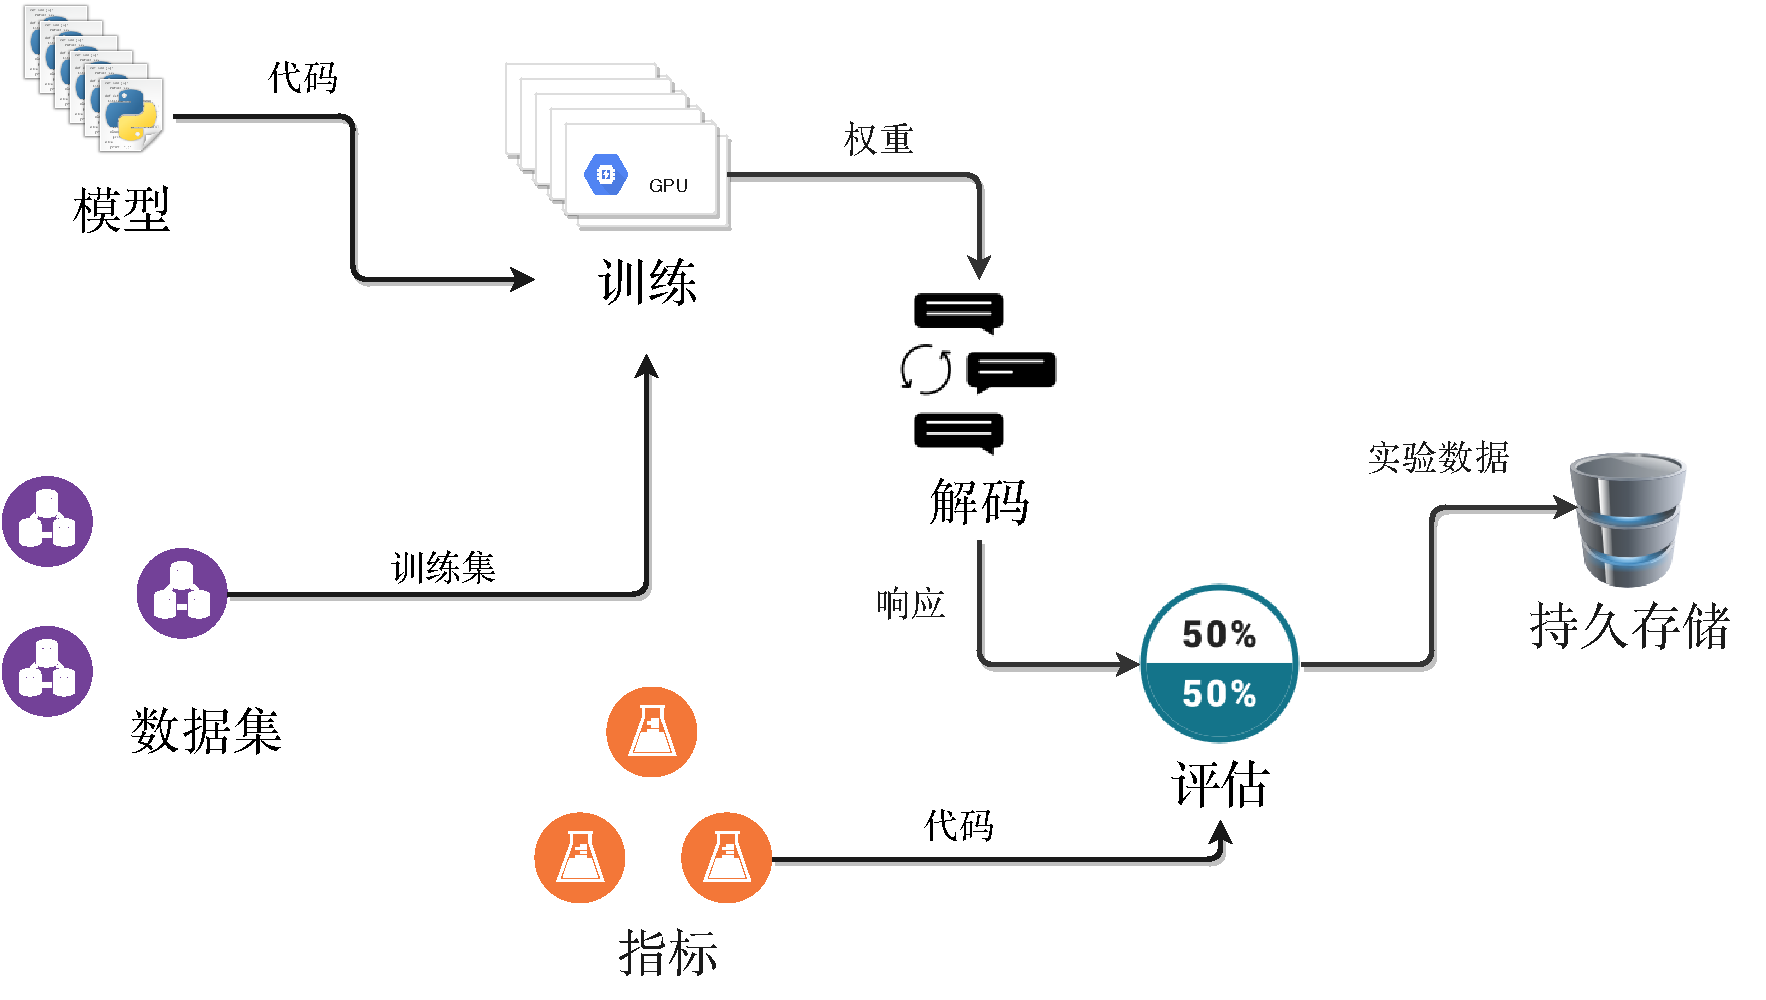
\includegraphics[width=0.8\textwidth]{figure/drawio/eval_v4.pdf}
    \caption{实验框架}
    \label{fig:framework}
\end{figure}

% why did you choose these models?
% Show me you really understand these model.
% Why the selection of models is important?
% Two reasons: 1. they are seq2seq based. we only investigate s2s.
% 2. they are trained on 2 corpuses before. Their transferability
\section{模型选取}\label{sec:model_selection}
第~\ref{ch:related_work}~章已经介绍了生成式模型的基本概念和数据集、指标的基本情况。
和相对有限的数据集和指标相比,生成式模型的数量众多,
光是我们了解到的不同的模型就有不下十几个。
由于时间有限,
我们把考察的范围限定在基于Seq2Seq框架的生成式模型。
Serban等人在\upcite{HRED,VHRED,MrRNN,A_Short_Review}
中提出或者使用了LSTM,HRED,VHRED和MrRNN等模型,
它们大多是Seq2Seq框架在体系结构上的扩展。
除了LSTM是作为基线的RNN语言模型外,这些模型都各具特色:
HRED能利用长期对话历史,
VHRED能捕捉对话中的不确定性(Uncertainty)和歧义性(Ambiguity),
MrRNN能生成带有高级组合结构(Compositional Structure)的响应。
而且,HRED和VHRED都在Ubuntu Dialogue Corpus和
Twitter Triple Corpus两个数据集上取得了不错的成绩,
说明它们在迁移能力方面是比较强的基线。
是否基于Seq2Seq框架和迁移能力是我们选择模型的两大依据,
HRED和VHRED很好的符合了我们的需求。

我们没有选取普遍的Seq2Seq模型作为基线,
而是选取了LSTM语言模型,因为它足够简单而且是一个非Seq2Seq结构,
作为基线模型已经足够好了。
我们把加入普通的Seq2Seq模型作为以后的工作。
下面将会详细介绍LSTM,HRED和VHRED三个模型。

% show the power of Serban
\subsection{LSTM语言模型}\label{subsec:LSTM}

\begin{align}
    f_t &= \sigma(W_f \cdot [h_{t-1}, x_t] + b_f) \\
    i_t &= \sigma(W_i \cdot [h_{t-1}, x_t] + b_i) \\
    \hat{C}_t &= \tanh(W_C \cdot [h_{t-1}, x_t] + b_C) \\
    C_t &= f_t \times C_{t-1} + i_t \times \hat{C}_t \\
    o_t &= \sigma(W_o \cdot [h_{t-1}, x_t] + b_o) \\
    h_t &= o_t \times \tanh(C_t)
\end{align}
\begin{figure}
    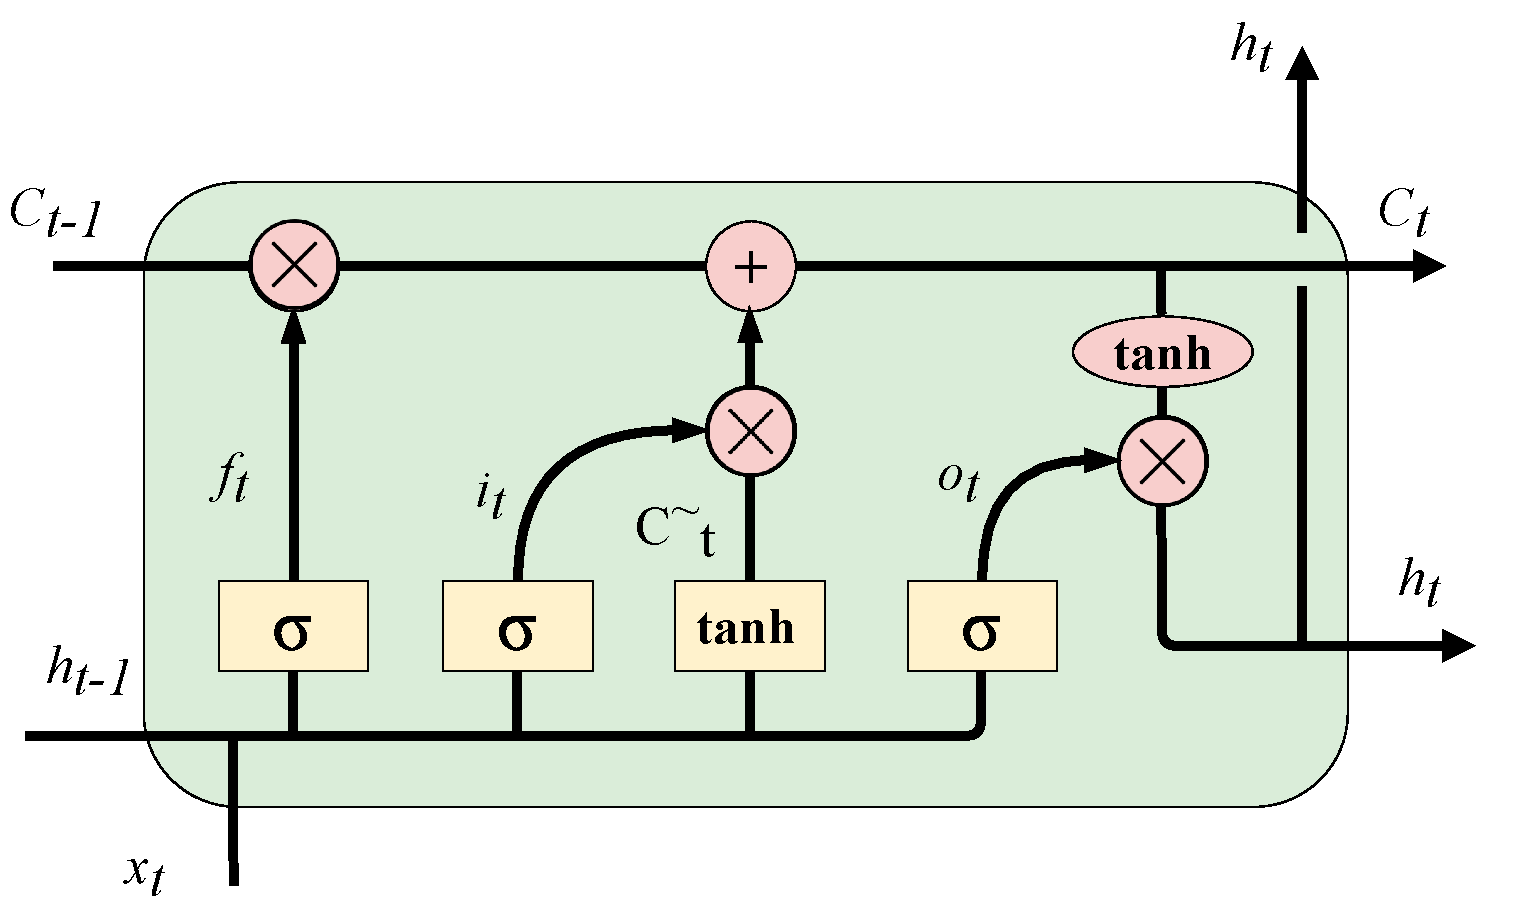
\includegraphics[width=0.6\textwidth]{figure/drawio/LSTM_v5.pdf}
    \centering
    \caption{LSTM内部连接图}
    \label{fig:LSTM_Internal}
\end{figure}

\subsection{HRED模型}\label{subsec:HRED}
多层编解码器(Hierarchical Recurrent Encoder-Decoder,HRED)\upcite{hred-qs}是一种能利用多轮对话结构的生成式模型。
它把一个对话看做一个两层序列结构:一个对话$D$由$M$个句子组成,每个句子由$N_m$个单词组成:
\begin{align}
    D &= \{ U_1, \cdots, U_M \} \\
    U_m &= \{ w_{m, 1}, \cdots, w_{m, N_m} \}
\end{align}

HRED由三个RNN组成:一个编码RNN(Encoder RNN)负责把每一个句子编码成一个固定长度的向量,称为句子向量(Utterance Vector);
一个上下文RNN(Context RNN)负责迭代的处理句子向量,
把直到并且包括当前轮$m$的所有轮的句子$U_1, \cdots, U_m$编码成一个对话向量(Dialogue Vector);
最后,一个解码RNN(Decoder RNN)负责以对话向量为条件,生成对话的下一个句子$U_{m+1}$。
三个RNN的协作关系如~图\ref{fig:HRED_computation_graph}~所示。
本质上,HRED通过把对话分解为句子的序列,
把句子分解为单词的序列,估计了一个对话$D$的概率$P_{\theta}(D)$:
\begin{align}
    P_{\theta}(D) &= P_{\theta}(U_1, \cdots, U_M) \\
    &= \prod_{m=1}^M P_{\theta}(U_m|U_{<m}) \\
    &= \prod_{m=1}^M \prod_{n=1}^{N_m} P_{\theta}( w_{m, n} |w_{m, <n}, U_{<m} )
\end{align}

$\theta$是HRED模型的参数,
$U_{<m}$表示$U_m$之前的句子序列:
$U_{<m} = \{ U_1, \cdots, U_{m-1} \}$,
$w_{m, <n}$表示第$m$个句子的第$n$个单词之前的单词序列:
$w_{m, <n} = \{ w_{m, 1}, \cdots, w_{m, n-1} \}$。

\begin{figure}[H]
    \centering
    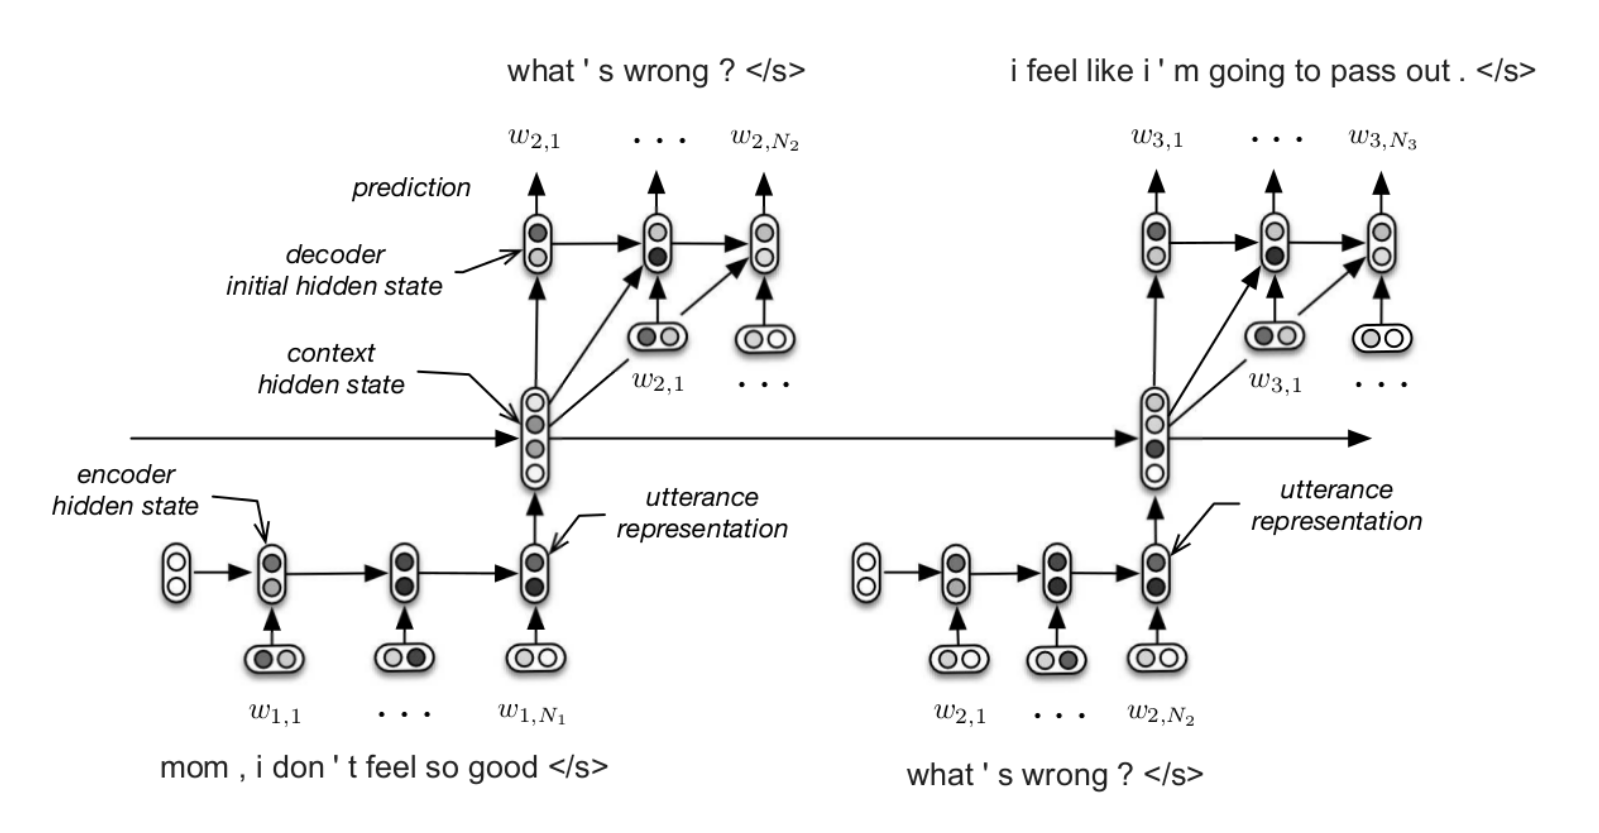
\includegraphics[width=\textwidth]{figure/HRED.png}
    \caption{HRED的计算图\upcite{HRED}}
    \label{fig:HRED_computation_graph}
\end{figure}

\subsection{VHRED模型}\label{subsec:VHRED}

\section{模型超参数设置}\label{sec:model_hparams}
% ------ Model setup ----------- %
在模型超参数方面,我们的设置大致和\upcite{VHRED}相同。
我们用Adam\upcite{AdamOpt}来优化所有模型,
一个小批(Mini-batch)处理20个样本。
% -- Dimension of Word Embeddings -- %
我们在Ubuntu上使用维度是300的词嵌入,
在OpenSubtitles和LSDSCC上使用维度是400的词嵌入。
% -- Hidden Units of Utterance Encoder -- %
HRED和VHRED的句子编码器(Utterance Encoder)
在Ubuntu上使用500个隐藏单元,
在OpenSubtitles和LSDSCC上使用1000个隐藏单元
\footnote{LSTM模型是一个语言模型,只有句子解码器。}。
% -- Hidden Units of Context Encoder -- %
HRED和VHRED的上下文编码器(Context Encoder)
在所有数据集上都使用1000个隐藏单元。
% -- Hidden Units of Utterance Decoder -- %
不同模型的句子解码器(Utterance Decoder)
在不同数据集上的隐藏单元数量
如表~\ref{tab:utterance_decoder_hidden_units}~所示。
一般根据数据集的特点来设置不同RNN的隐藏单元数量,
在样本数多或者词汇表大的数据集上训练时,
隐藏单元数量会相应的增多。

% -- Direction of Utterance Encoder -- %
Ubuntu上的模型的句子编码器都使用了单向RNN,
而OpenSubtitles和LSDSCC上的模型的句子编码器则使用双向RNN。
% -- Gate Type of Utterance & Context Encoder -- %
所有模型的句子编码器和上下文编码器(如果有)都使用GRU作为门单元。
% -- Gate Type of Decoder -- %
句子解码器的门单元类型如表~\ref{tab:utterance_decoder_gate_types}~所示
\footnote{OpenSubtitles和LSDSCC上的LSTM模型的解码器都没有使用LSTM门单元,不过它们仍然是语言模型。}。
\begin{table}
    \centering
    \caption{句子解码器的配置情况}
    \setlength{\tabcolsep}{0.11cm}%
    \begin{subtable}{0.5\linewidth}
        \centering
        \caption{门单元类型}
        \label{tab:utterance_decoder_gate_types}
        \begin{tabular}{llll}
            \toprule
            \midrule
            & HRED & LSTM & VHRED \\
            \midrule
            LSDSCC & LSTM & GRU & GRU \\
            OpenSubtitles & LSTM & GRU & GRU \\
            Ubuntu & LSTM & LSTM & LSTM \\
            \bottomrule
        \end{tabular}
    \end{subtable}%
    \begin{subtable}{0.4\linewidth}
        \centering
        \caption{隐藏状态单元数量}
        \label{tab:utterance_decoder_hidden_units}
        \begin{tabular}{lll}
            \toprule
            \midrule
            HRED & LSTM & VHRED \\
            \midrule
            1000 & 2000 & 1000 \\
            1000 & 2000 & 1000 \\
            500 & 2000 & 500 \\
            \bottomrule
        \end{tabular}
    \end{subtable}
\end{table}

所有的模型都在一台GeForce GTX TITAN X上训练了至少1周。
模型收敛时的困惑度如表~\ref{tab:converged_perplexity}~所示。
与\upcite{VHRED}不同的是,我们没有用预训练的HRED的参数来初始化对应的VHRED。
所有的模型都使用了梯度剪裁,阈值为1。
所有模型在Ubuntu上的学习率为0.0002,
在OpenSubtitles和LSDSCC上的学习率为0.0001。
在解码时,我们使用随机取样。
\begin{table}
    \centering
    \caption{模型收敛时的困惑度}
    \label{tab:converged_perplexity}
    \begin{tabular}{llll}
        \toprule
        \midrule
        & HRED & LSTM & VHRED \\
        \midrule
        LSDSCC & 32.9229 & 32.5599 & 37.7149 \\
        OpenSubtitles & 41.6392 & 34.2724 & 33.6867 \\
        Ubuntu & 39.1623 & 46.4055 & 40.2486 \\
        \bottomrule
    \end{tabular}
\end{table}

% -- Dataset Preprocessing -- %
\section{数据集预处理}
\label{sec:dataset_proprecessing}
我们使用的Ubuntu Dialogue Corpus直接来自Serban等人的项目
\footnote{\url{https://github.com/julianser/hed-dlg-truncated.git}},没有经过任何额外处理。
我们从Li等人的项目
\footnote{\url{https://github.com/jiweil/Neural-Dialogue-Generation.git}}
中获取了经过预处理的OpenSubtitles数据,并作了如下处理:
\begin{enumerate}
    \item 将其从整数的下标形式还原为字符串的单词形式;
    \item 将其词汇表文件\texttt{movie\_25000}转化为下标从0开始的 pickle\footnote{pickle是一个Python特有的序列化格式}格式。
    \item 用Serban等人的\texttt{convert\_text2dict.py}将训练集,
    测试集和开发集均转换为pickle格式;
    \item 选用OpenSubtitles中的轮数为3, 句子最短长度为6的dialogue3\_6格式作为实际使用的数据集;
    \item 从测试集随机抽取1\%的样本作为正式使用的数据集。
\end{enumerate}

LSDSCC也是一个经过预处理的数据集\footnote{\url{https://drive.google.com/file/d/1nbpbnhwNP14xAc4SAc1 NN5lvEr01dQb/view?usp=sharing}}。
由于它的词汇数量多达50K,为了使内存不至于溢出,我们将其词汇表裁剪至35000个最常见的单词。
此外,由于我们只使用单个参考的指标,因此对LSDSCC的测试集中的多个参考,我们只取第一个参考。
剩下的处理过程类似OpenSubtitles的处理。

表~\ref{tab:train_set_stats}~是三个数据集的训练集的一些统计数据。
从表中可以看到,OpenSubtitles的样本数量要远远超过其他两个数据集,
是Ubuntu的26倍, 是LSDSCC的16倍。
但是,从单词数量来看,OpenSubtitles超过另外两个数据集的倍数却小得多,
这是因为Ubuntu的每一个样本包含了多个句子,
其长度要远远超过OpenSubtitles的样本。
这也导致了Ubuntu的样本数量少于LSDSCC,但是单词数量却超过了LSDSCC。
测试集的统计数据如表~\ref{tab:test_set_stats}~所示。
对于LSDSCC的测试集,我们其实可以从其训练集分一部分出来作为测试集,
这样可以使样本数量更多。
但是,为了是训练集尽可能大,
我们选择了从LSDSCC的多重参考测评集中构造测试集,
导致测试集的样本只有不到300个。
\begin{table}[H]
    \centering
    \caption{数据集的统计数据}
    \begin{subtable}{0.6\linewidth}
        \centering
        \caption{训练集}
        \label{tab:train_set_stats}
        \begin{tabular}{lllll}
            \toprule
            \midrule
            数据集 & 词汇数量 & 样本数量 & 单词数量 & 轮数 \\
            \midrule
            Ubuntu & 20000 & 448833 & 45697699 & 多轮 \\
            OpenSubtitles & 23876 & 11771393 & 379346841 & 多轮 \\
            LSDSCC & 35008 & 738095 & 32355628 & 单轮 \\
            \bottomrule
        \end{tabular}
    \end{subtable}%
    \begin{subtable}{0.3\linewidth}
        \centering
        \caption{测试集}
        \label{tab:test_set_stats}
        \begin{tabular}{lll}
            \toprule
            \midrule
            样本数量 & 单词数量 \\
            \midrule
            18920 & 2045082   \\
            14714 & 474074 \\
            299 & 10914 \\
            \bottomrule
        \end{tabular}
    \end{subtable}
\end{table}

% -- Metric Config -- %
\section{指标配置}\label{sec:metric_config}
我们尽可能使用业界公认的指标实现和推荐的指标参数。
和\upcite{HowNot}一样,我们只考虑单轮对话,
并且每个系统输出响应都只有单个参考响应。
% -- BLEU -- %
我们使用NLTK\footnote{\url{https://www.nltk.org/}}提供的BLEU实现,
并且加入了平滑处理。
% -- ROUGE -- %
我们实现了的ROUGE的一个版本,并将准确率和召回率的比例设置为1:9,
因为在机器翻译领域,
召回率和人类评价的相关性比准确率高\upcite{METEOR}。
ROUGE-W的权重设置为1.2 。
% -- METEOR -- %
我们使用了METEOR的官方实现\texttt{meteor-1.5.jar},并且按照官方文档
\footnote{\url{http://www.cs.cmu.edu/~alavie/METEOR/README.html}}的说明,
加入对特定语言(英语)的正则化处理。
% -- PPL -- %
我们使用Serban等人的\texttt{evaluate.py}脚本测量模型的困惑度,
由于该程序对测试样本进行了随机取样,我们无法得知某个样本的确切得分,
所以只测得了系统层面的得分。
% -- EB -- %
关于词嵌入的指标,
我们改写了Serban等人的\texttt{embedding\_metrics.py},
使之能测量句子层面的得分;
和他们一样,我们使用在谷歌新闻文库(Google News Corpus)上预训练的
word2vec词嵌入\footnote{\url{https://drive.google.com/file/d/0B7XkCwpI5KDYNlNUTTlSS21pQmM}}。
% -- ADEM -- %
关于ADEM指标,我们使用作者提供的代码库
\footnote{\url{https://github.com/mike-n-7/ADEM.git}}
和预训练模型\footnote{\url{https://drive.google.com/file/d/0B-nb1w_dNuMLY0Fad3N1YU9ZOU0/view?usp=sharing}}。
% -- Distinct-N -- %
我们实现了比较简单的Distinct-N指标。
我们还测量了响应的句子长度$\textit{\#words}$,
以观察它对不同指标的得分的影响。

\section{本章小结}\label{sec:method_conclusion}
本章详细介绍了实验的各项设置,包括模型的超参数和训练过程,
数据集的预处理操作和一些统计数据,以及指标的实现和参数选择。
在下一章中,我们将展示实验的结果并进行讨论。
